% SECTION 15: Phase Transitions in the Lattice Theory
% Source: extract/sec15.txt (PDF pages 93-97) + continuation at the head of
% extract/sec16.txt (PDF page 98, before the "16. Errors in Lattice Results" heading).

\chapter{Phase Transitions in the Lattice Theory}

The lattice theory with a finite cut-off $\mu = \pi/a$ can be regarded as an effective theory. The integration over momenta in the range $\{\pi/a, \infty\}$ renormalizes the couplings and generates additional effective interactions (see Section 8 and the lectures by M.~L\"uscher for a detailed discussion of this approach). Thus, one can regard the lattice theory as a point in an infinite dimensional space of couplings, and taking the continuum limit as a flow in this space to the critical point at $a = 0$ that defines the physical theory. In this way of thinking about LQCD as a Statistical Mechanics system one is automatically lead to the questions
\begin{itemize}
\item What is the phase diagram in this extended coupling constant space?
\item Are there other fixed points, and if so what is the nature of the theory at those points?
\item What are the order parameters that characterize different phases?
\end{itemize}

The starting point of my discussion of these questions will be the pure gauge theory. As before, the generalized form of the gauge action is
\begin{equation}
S_g = \beta \sum_{i,j} \sum_{\mu,\nu} \sum_x c_{i,j}\, \mathrm{Re}\, \mathrm{Tr}\, W^{i,j}_{\mu\nu}
\end{equation}
where the sum over $i$ in $W^{i,j}_{\mu\nu}$ is over all possible Wilson loops and $j$ is over all representations of the loop. $\beta$ is the overall coupling and the $c_{i,j}$ give the relative strengths of the different loops.

The three simplest gauge invariant probes of the phase diagram are (gauge non-invariant quantities have zero expectation values as shown by Elitzur [37])
\begin{itemize}
\item Wilson loops: These, as discussed in Section 14.2.1, contain information on the potential between static quarks.
\item Wilson/Polyakov lines. These measure the free energy of an isolated quark.
\item The chiral condensate $\langle \bar{\psi}\psi\rangle$. This provides information on vacuum alignment under spontaneous chiral symmetry breaking.
\end{itemize}

LQCD, in the limit $g \to \infty$, can be analyzed using strong coupling expansions as discussed in Section 14.2.2. Using these it was shown that, in the limit $g \to \infty$, the expectation value for Wilson loops has an area law for all gauge groups ($U(1)$ and $SU(N)$). Since electrodynamics ($U(1)$) does not confine, this region of coupling space cannot correspond to the physical theory. In other words, there should exist a phase transition separating the strong coupling and weak coupling phases of non-confining theories like $U(1)$. This has been established for $U(1)$, both analytically [130] and by Monte Carlo simulations [131]. For a theory like QCD, with both confinement and asymptotic freedom, we need to know if the two regions of parameter space are analytically connected. Analytical methods like strong and weak coupling expansions can be used provided the range of validity of the expansions gives a sufficiently large overlap, otherwise non-perturbative methods are necessary.

To address these questions for $SU(3)$ I show, in Fig.~\ref{fig:14}, the behavior of square loops, $\{\mathrm{Re}\,\mathrm{Tr}\, W^{i \times i}\}$, as a function of the coupling $\beta$ for the simplest action---Wilson's plaquette action. Also shown for comparison are the strong coupling expansion to $O(\beta^5)$ [133], the weak coupling expansion to $O(g^4)$ [134] and its tadpole improved (TIPT) version. These numerical data show that there is a smooth though sharp transition between the weak coupling and strong coupling phases, i.e.~no phase transitions. The crossover takes place in the window $5 \lesssim \beta \sim 6$, with the larger loops becoming perturbative at slightly higher $\beta$. Both strong coupling and weak coupling expansions fail in this region (for TIPT this is evident only for large loops), so numerical methods are essential. Such an analysis was the basis of the pioneering work of Creutz, and Creutz, Jacobs, and Rebbi [132], who showed that the string tension changes from its strong to weak coupling behavior without a phase transition. Their calculations yielded the first clue that it may be possible to get continuum physics with $O(20\%)$ errors from simulations at $\beta \gtrsim 6.0$.

\begin{figure}[htbp]
\centering
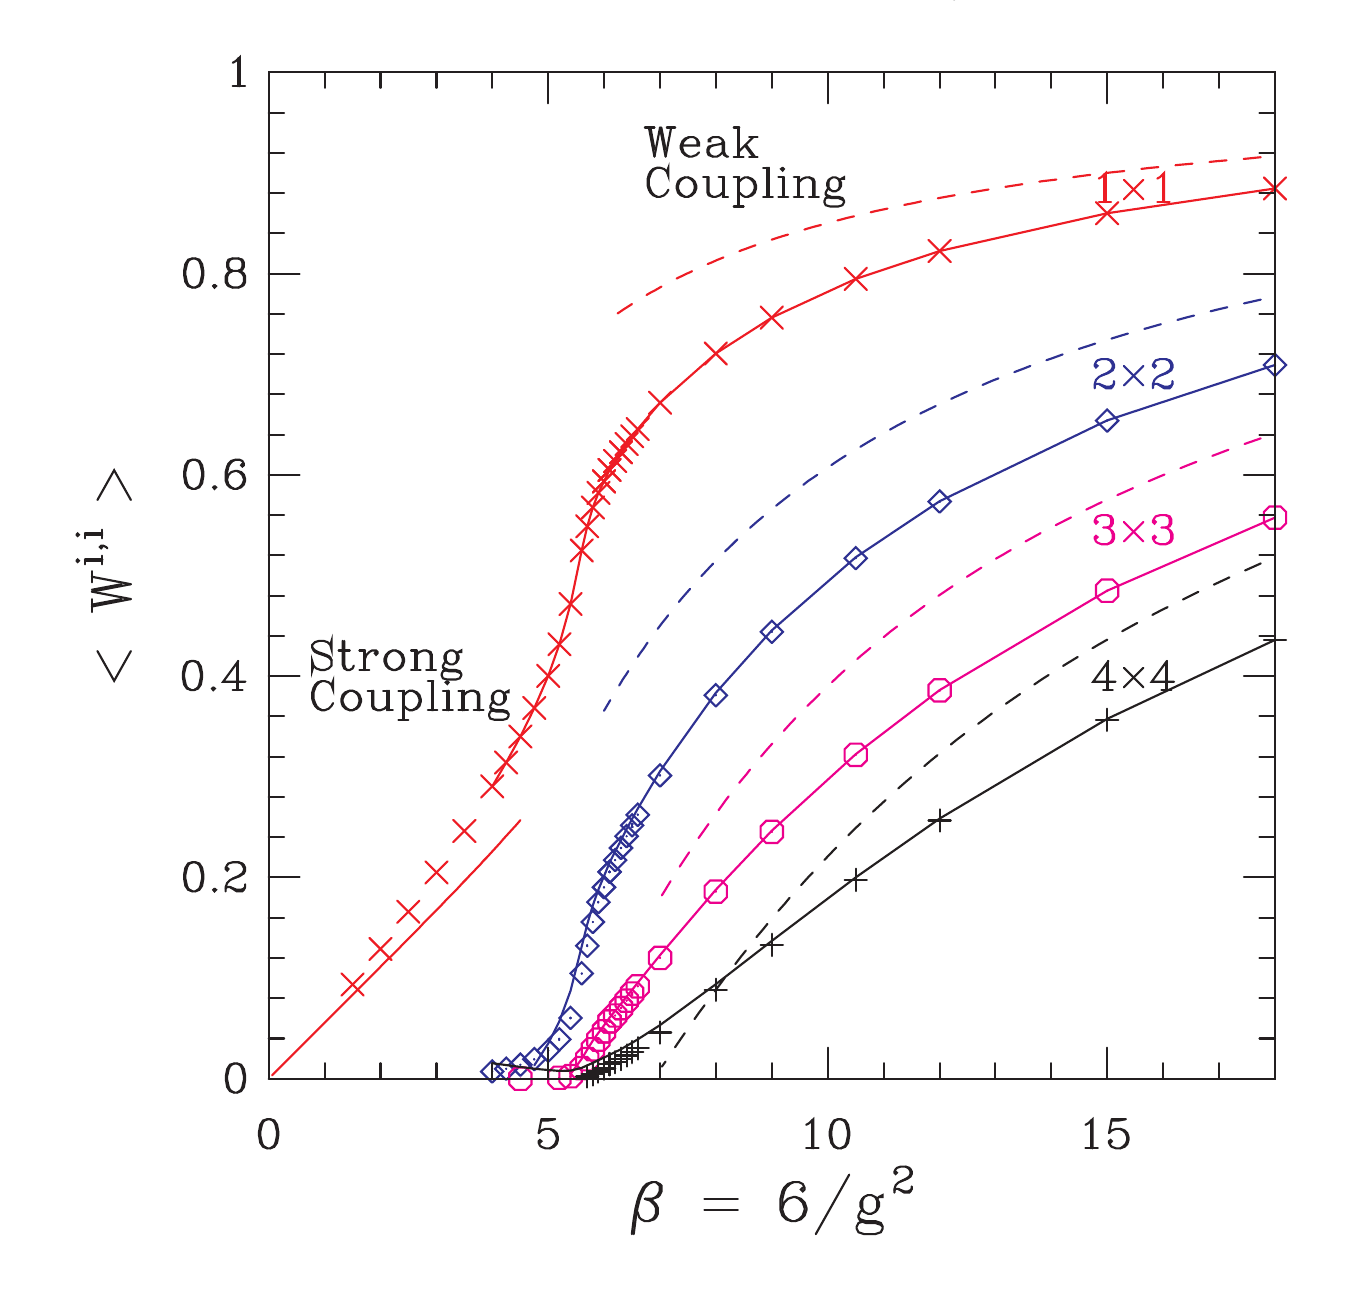
\includegraphics[width=0.8\textwidth]{images/fig14.png}
\caption{The behavior of the expectation value of square Wilson loops as a function of coupling $\beta$. The data, show a sharp crossover between $5 \lesssim \beta \lesssim 6.0$. Result of the strong coupling expansion to $O(\beta^5)$ and weak coupling expansion to $O(g^4)$ are shown by the dashed line. Results of tadpole improved weak coupling expansion (TIPT) are shown by the solid lines. Since the improved coupling is defined in terms of the $1 \times 1$ loop, $g_I^2 = g^2/\langle W^{1 \times 1}\rangle$, the agreement between the data and TIPT is a trivial result of the construction as explained in the text. The improvement in larger loops, however, demonstrates the efficacy of TIPT.}
\label{fig:14}
\end{figure}

The TIPT result shown in Fig.~\ref{fig:14} is obtained as follows. The mean-field improved Wilson loop expectation value is defined to be
\begin{equation}
\langle W^{i \times i}\rangle = \langle \tilde{W}^{i \times i}\rangle\, u_0^{4i},
\end{equation}
where for $u_0$ I use the non-perturbative value obtained from the plaquette as it is more readily available. The improved expansion for $\langle \tilde{W}^{i \times i}\rangle$, after absorbing the tadpoles using the plaquette, is given by
\begin{equation}
\langle \tilde{W}^{i \times i}\rangle = \frac{\langle W^{i \times i}\rangle}{\langle W^{1 \times 1}\rangle^i},
\end{equation}
where both terms on the right are first expanded in terms of $\tilde{g}^2 = g^2/u_0^4(\mathrm{pert}) = g^2/\langle W^{1 \times 1}\rangle_{\mathrm{pert}}$ to order $\tilde{g}^4$, and then the ratio is truncated at order $\tilde{g}^4$. It is obvious that using $u_0$ from the plaquette guarantees a perfect fit for $\langle W^{1 \times 1}\rangle$, however the improvement in even the $\langle W^{4 \times 4}\rangle$, is remarkable.

The first study of the phase diagram in the generalized coupling constant space was done using an action constructed from the plaquette in both the fundamental and adjoint representations of the $SU(N)$ gauge theory [135]
\begin{equation}
S = \beta_F \sum_x \frac{1}{N} \mathrm{Re}\, \mathrm{Tr}\, W_{1 \times 1} + \beta_A \sum_x \frac{1}{N^2} |\mathrm{Tr}\, W_{1 \times 1}|^2 .
\end{equation}
For this action, the effective bare coupling, obtained using a Taylor expansion, is
\begin{equation}
\beta_{\mathrm{eff}} \equiv \frac{2N}{g_{\mathrm{eff}}^2} = \beta_F + 2\beta_A .
\end{equation}
Thus simulations can be done in the negative $\beta_A$ region as long as $\beta_F > 2|\beta_A|$. This is a classical condition that avoids the weak coupling singularity.

The resulting lines of first order bulk transitions, along with the location of the end point for three gauge groups, are show in Fig.~\ref{fig:15}. The point at $\beta_A = \infty$ is the first order transition in the $Z(N)$ gauge theory, while that at $\beta_F = 0$ corresponds to that in the $SO(N)$ theory. The location of the third end-point with respect to the $\beta_F$ axis depends on $N$. Current estimates of the location are [136--138]
\begin{equation}
\begin{array}{lll}
\beta_F = 1.22 & \quad \beta_A = 1.25 & \quad \mathrm{SU}(2) \\
\beta_F = 4.00(7) & \quad \beta_A = 2.06(8) & \quad \mathrm{SU}(3) \\
\beta_F \sim 12{-}15 & \quad \beta_A = (-1) - (-5) & \quad \mathrm{SU}(4)
\end{array}
\end{equation}

The fact that for $N \le 3$ this point lies above the $\beta_F$ axis is consistent with the observation that there is no discontinuity in the behavior of Wilson loop data as show in Fig.~\ref{fig:14}. If one were to take the continuum limit along a line crossing the transition line above this point, for example along the dotted line $A$ in Fig.~\ref{fig:15}, then there would be discontinuities in Wilson loops (and consequently in the string tension), specific heat, and glueball masses at the point of intersection with the transition line. At the end-point $X$ the specific heat diverges and consequently the $0^{++}$ glueball mass goes to zero. (Note that the specific heat is the volume integral of the $0^{++}$ glueball correlation function with the plaquette as the interpolating operator. Thus the divergence in the specific heat implies a zero in the $0^{++}$ glueball mass.) The string tension and masses of glueball states with other spin-parity quantum numbers are non-zero and continuous at this point. Such phase transitions are lattice artifacts. For example, taking the continuum limit at $X$, i.e.~setting $a = 0$, would give a free theory as all states other than the $0^{++}$ glueball become infinitely heavy.

\begin{figure}[htbp]
\centering
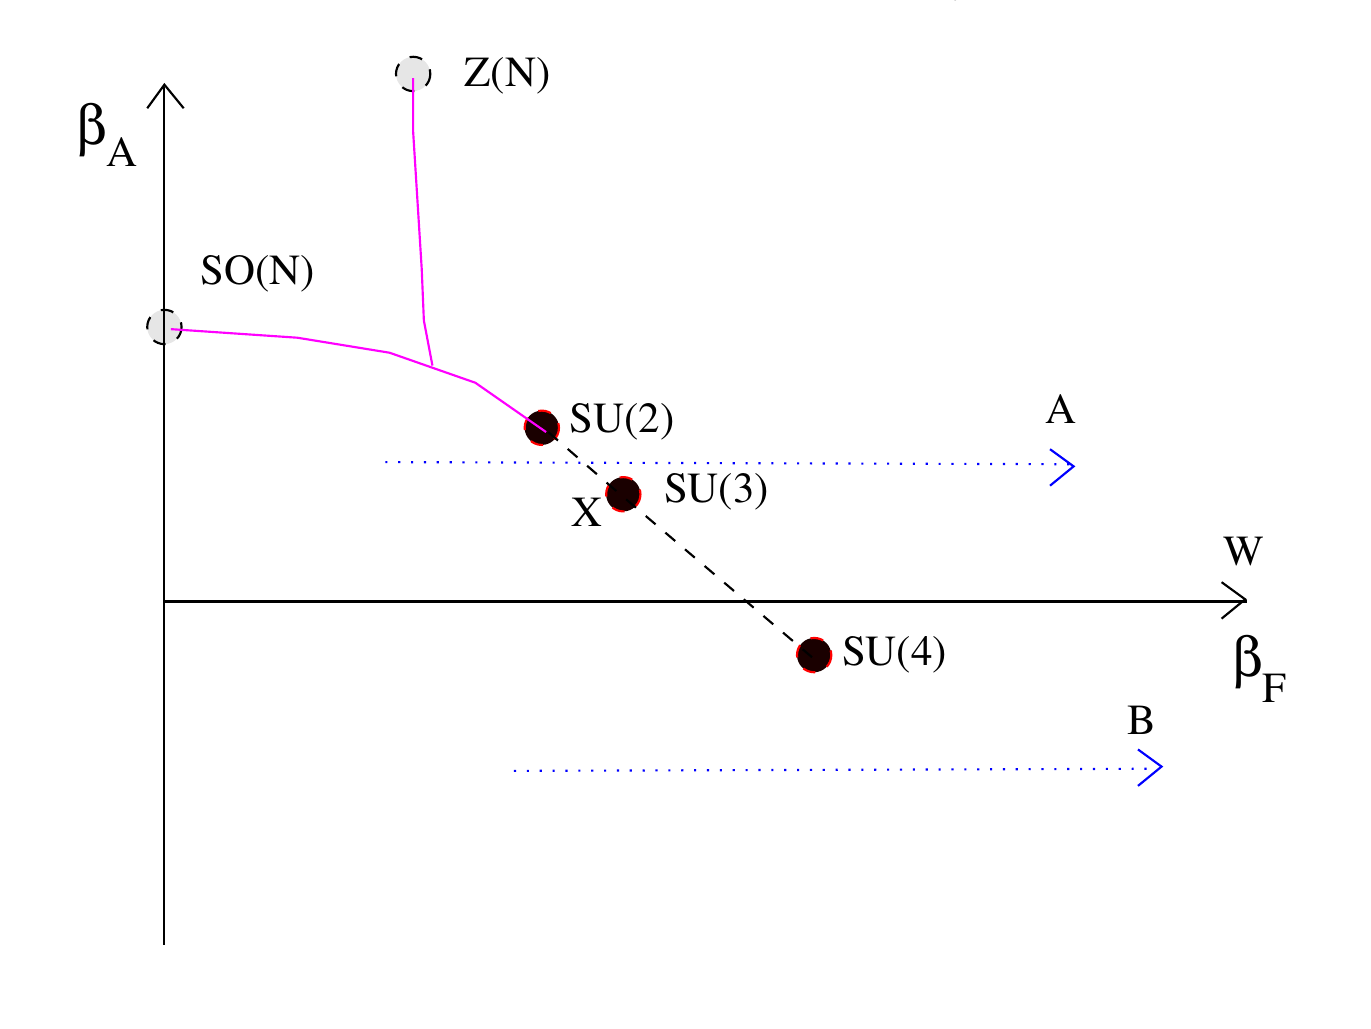
\includegraphics[width=0.8\textwidth]{images/fig15.png}
\caption{The phase diagram of $SU(N)$ gauge theories in the fundamental-adjoint coupling constant space.}
\label{fig:15}
\end{figure}

One can take the continuum limit for the $SU(3)$ gauge theory along any trajectory like $A$ or $W$ or $B$. In case $A$ it is necessary to keep $\beta_F > \beta_F^*$ to avoid the lattice artifacts. Along $W$, while there are no singularities, the artifact $X$ could, around $\beta_F = 5.7$, cause significant deviations from the physics of the relevant fixed point at $g = 0$. Lattice data verify this scenario---the non-perturbative $\beta$-function measured from observables other than $M_{0^{++}}$ shows a large dip around $\beta_F = 5.7$ [89]. Thus, to avoid these artifacts requires simulations for $\beta_F \gtrsim 6.0$. On a trajectory like $B$ the influence of $X$ is expected to be less than along $W$, and it is possible that contact with continuum physics can be made on coarser lattices. If so then the trajectory $B$ corresponds to an ``improved action'' in accordance with the third criteria enumerated in Section 8.

This qualitative argument for taking the continuum limit along a trajectory like $B$ is supported by Monte Carlo renormalization group (MCRG) estimates of the renormalized trajectory [87]. Such calculations of the RT yield a negative value for $\beta_A$. As explained above, the most sensitive probe of the expected improvement on including a $\beta_A$ term in the action, is the behavior of $M_{0^{++}}$. Until recently tests of this conjecture were limited by statistical accuracy [166]. The recent calculations on anisotropic lattices of glueball spectra by Morningstar and Peardon [139] validate this scenario. I shall discuss their results in Section 18.3.

It is clear that there are additional phase transitions in the generalized lattice theory. For example one would get a similar diagram to that in Fig.~\ref{fig:15} if the action was defined in terms of the $1 \times 2$ loop in the fundamental and adjoint representations. The question, therefore, is whether there exist other second order transition points at which all correlation lengths (measured in lattice units) diverge i.e.~where a non-trivial continuum limit exists. The commonly held belief, supported by numerical data, is that all such points lie on the hypersurface defined by $g_{\mathrm{eff}} = 0$. The long distance behavior of these theories is controlled by the fixed point defined with respect to a suitable renormalization group transformation. Taking the continuum limit of the lattice theory on this hypersurface provides a non-perturbative definition of QCD. This is the standard scenario.

An alternative scenario is the presence of a non-trivial fixed point at $g_{\mathrm{eff}} \neq 0$ [140]. If this unlikely possibility turns out to be true then the perturbative relation between $g_{\mathrm{eff}}$ and $a$, based on asymptotic freedom, would change---the coupling would no longer run to zero as the momentum scale $Q \to \infty$. This could be exposed by precise measurements of $\alpha_s$ as a function of $Q^2$, or by a detailed search for non-trivial second order phase transitions in the lattice theory.

In either case the non-perturbative lattice analyses of quantities such as the spectrum and weak matrix elements does not change. To get to the continuum limit we would still extrapolate the lattice data in $a$ to $a = 0$. Only the PQCD relation between $a$ and $g$ would be invalid, consequently extrapolations using the perturbative scaling relation could not be used.

My bottom line on this issue, having mentioned the heretical view, is to proceed assuming that the standard scenario is correct.
